% \chapter{An alternative translational start \texorpdfstring{site \\identified}{site identified} in \texorpdfstring{\(PPARG\)}{PPARG} generates \texorpdfstring{a \\functional}{a functional} isoform
\chapter{An alternative translational start site identified in PPARG generates a functional isoform
}\label{chap:chapter 1}

%%%%%%%%%%%%%%%%%%%%%%%%%%%%%%%%%%%%%%%%%%%%%%%%%%%%%%%%%%%%%%%%%%%%%%%%%%%%%%%%
\section{Introduction}
%%%%%%%%%%%%%%%%%%%%%%%%%%%%%%%%%%%%%%%%%%%%%%%%%%%%%%%%%%%%%%%%%%%%%%%%%%%%%%%%

Insulin resistance is a major driver of the epidemic diseases, type 2 diabetes, cardiovascular disease (CVD), and nonalcoholic fatty liver disease (NAFLD), that challenge global health\cite{James2021-vu,Adeva-Andany2019-df,Khan2019-qt}. Thiazolidinediones (TZDs) are a class of drugs that decrease insulin resistance by agonizing PPAR$\gamma$\cite{Yki-Jarvinen2004-ba}, a nuclear hormone receptor that contains an autonomous activation-function domain 1 (AF-1), DNA binding domain (DBD), and ligand binding domain (LBD) (\textbf{Figure 1.1A})\cite{Tontonoz1994-nk}. TZDs have demonstrated clinical efficacy in treating type 2 diabetes, CVD, and NAFLD\cite{Kernan2016-fd,Inzucchi2016-ni,Musso2017-xi}, but their use has been limited by serious side effects, such as weight gain and fluid retention, which are a direct consequence of PPAR$\gamma$ agonism through interaction at its ligand-binding domain (LBD)\cite{Yki-Jarvinen2004-ba}. Much pharmacological development has been focused on the development of selective PPAR$\gamma$ modulators (SPPARMs) that retain the benefits of TZDs without the attendant adverse effects, but successful compounds have not reached the clinic\cite{Higgins2010-tv,DePaoli2014-hi}. Thus, the need for alternative approaches to therapeutically activate PPAR$\gamma$ without PPAR-mediated side effects remains unmet.

In this study, we report a novel protein isoform of PPAR$\gamma$ (named PPAR$\gamma$ M135), which lacks the AF-1 domain and is generated from an alternative translational start site (hg38:chr3:12381414). Through biochemical and transcriptomic profiling, we find that PPAR$\gamma$ M135 demonstrates enhanced ligand-inducible transcriptional and functional activity compared to wild-type (WT), leading us to a model of de-repression by loss of AF-1.

%%%%%%%%%%%%%%%%%%%%%%%%%%%%%%%%%%%%%%%%%%%%%%%%%%%%%%%%%%%%%%%%%%%%%%%%%%%%%%%%
\section{Results}
%%%%%%%%%%%%%%%%%%%%%%%%%%%%%%%%%%%%%%%%%%%%%%%%%%%%%%%%%%%%%%%%%%%%%%%%%%%%%%%%

\subsection{A novel functional PPAR\texorpdfstring{$\gamma$}{gamma} isoform, M135, is generated from an alternative translational start site}

In our initial experiments the endogenous \(PPARG\) locus was systematically disrupted by inducing insertions and deletions (indels) in each coding \(PPARG\) exon in a human macrophage cell line (THP-1), a tractable model suitable for large scale genetic perturbation that we and others have shown phenocopy \(PPARG\) related transcriptional responses in adipocytes\cite{Majithia2016-bm,Agostini2018-bx}. Findings from THP-1s were confirmed and extended in human adipocytes models, the physiologically relevant cell type for metabolic disease. The effect of \(PPARG\) disruptions was measured by quantifying the ability of the resulting cells to transactivate CD36, a direct PPAR$\gamma$ transcriptional target\cite{Tontonoz1998-aq}. A custom lentiviral library of CRISPR/Cas9 constructs with guides (sgRNAs) targeting all coding exons, untranslated regions, and introns (n=95), was introduced into THP-1 monocytes at one construct per cell. The resulting population of genome-edited cells was differentiated into macrophages, stimulated with 1 $\mu$M PPAR$\gamma$ agonist rosiglitazone, and sorted by FACS according to the expression of CD36 (\textbf{Figure 1.1B}). The CD36+ and CD36- populations were sequenced to recover the identities of the sgRNAs, and an enrichment score (ES) was calculated based on the counts of each sgRNA in the CD36+/CD36- pools (\textbf{Figure 1.1B, C}). Intron targeting sgRNAs introduced as controls had an average ES of 0.487. As expected, targeting sgRNAs to Exon B of \(PPARG\) (specific to the PPAR$\gamma$2 isoform) did not reduce CD36 activity ($\overline{ES}$=0.622), and most sgRNAs targeted to exons downstream of the PPAR$\gamma$1 start site caused severe loss of CD36 transactivation ($\overline{ES}$=-1.33). Intriguingly, five sgRNAs targeting Exon 1 of \(PPARG\), downstream of the PPAR$\gamma$1 start site, which would be predicted to maximally disrupt the protein sequence, had little effect on CD36 transactivation ($\overline{ES}$=0.629), suggesting an intact PPAR$\gamma$ response in the cells that harbored them (\textbf{Figure 1.1C}).  

\clearpage
\begin{figure}[!t]
    \centering
    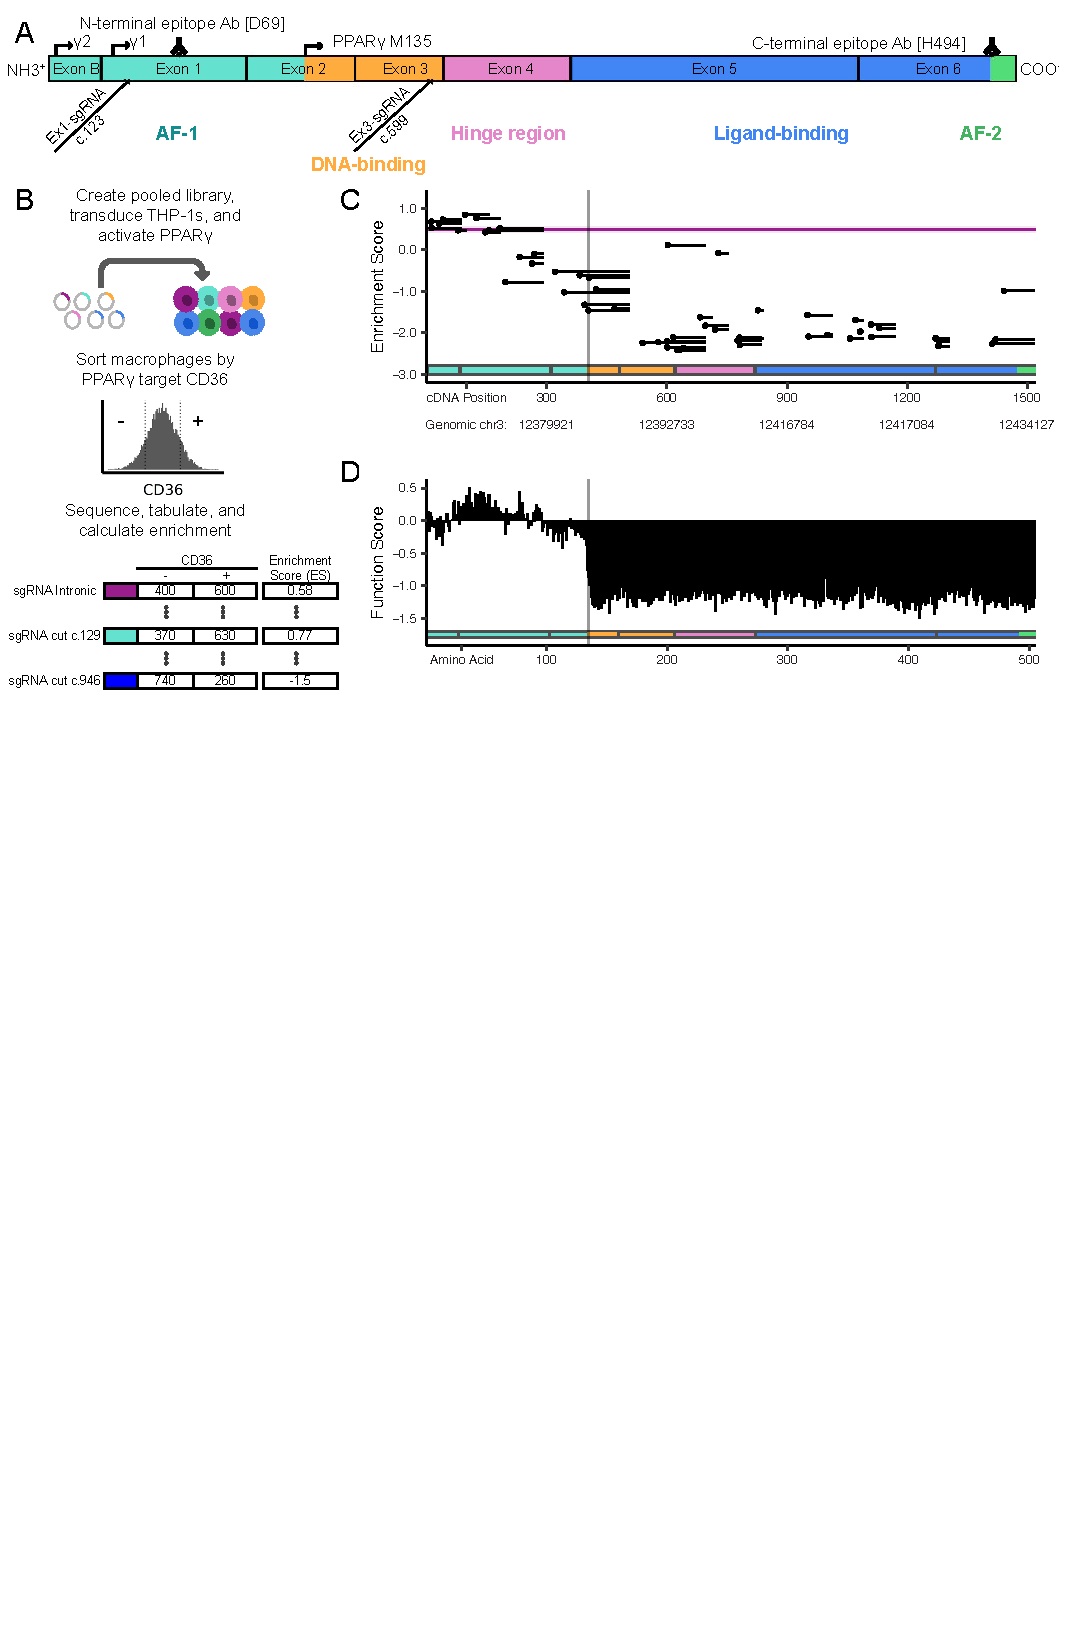
\includegraphics[width=\textwidth]{1_figures-and-files/Fig1.pdf}
    \caption[Functional screens across \(PPARG\) reveal an alternative translational start site at p.M135.]{\textbf{Functional screens across \(PPARG\) reveal an alternative translational start site at p.M135.} A. Linear representation of PPAR$\gamma$ indicating start sites for $\gamma$1, $\gamma$2 and novel M135. Guides and cut sites (Ex1-sgRNA; chr3:12379745 and Ex3-sgRNA; chr3:12392733. hg38) of CRISPR/Cas9 monoclonal generated cells are shown. Domain structure of PPAR$\gamma$ protein is represented in colors, and epitopes of the N-terminus and C-terminus antibodies (Abs) are indicated.  B. A library of 95 guide RNAs (sgRNAs) targeting \(PPARG\) was generated and transduced into THP-1 monocytes, such that each cell received a single construct. The polyclonal THP-1s were differentiated into macrophages, stimulated with a PPAR$\gamma$ agonist, 1 uM rosiglitazone (rosi), and sorted by FACS for expression of PPAR$\gamma$ target CD36 into bins of low (-) and high (+) PPAR$\gamma$ activity (n=5 independent replicate sorts). C. Enrichment scores (ES) from the CRISPR screen across PPARG. The mean ES for each guide across the 5 sort replicates is plotted along the PPARG2 cDNA based on its cut site (dot) and predicted termination after a 1 base indel (line). The horizontal purple line is the mean and standard error (se) of the intronic guides (n=18). PPAR$\gamma$ p.M135 is denoted by the vertical line. D. Function scores (FS) of insertions/deletions (indels) at each amino acid of PPAR$\gamma$2 calculated as previously published (Majithia et al. 2016). FS=0 refers to wild-type activity.
    }\label{fig:1 Alternative translational start site identification}
\end{figure}

To further understand this unexpected finding, we analyzed data generated from a previously conducted saturation mutagenesis study of \(PPARG\) that contained indels at every codon of the PPAR$\gamma$2 cDNA (CCDS2609; \textbf{Figure 1.1D})\cite{Majithia2016-bm}. Most indels that caused frameshift terminations in \(PPARG\) resulted in complete abrogation of rosiglitazone-induced CD36 transactivation, as evidenced by negative function scores (FS, Figure 1.1D). However, frameshifting indels in the 5$^{\prime}$ region of the cDNA, which would be predicted to cause very early termination of protein translation through nonsense disruption of the open reading frame, paradoxically retained cellular PPAR$\gamma$ transactivation ($\overline{FS}$=0.0322). This concurred with our finding of tolerated Exon 1 disruptions at the endogenous \(PPARG\) locus (Figure 1.1C) and suggested a possible post-splicing mechanism for retained PPAR$\gamma$ activity. The tolerance to early frameshifting indels was observed until c.A403 (CCDS2609), after which frameshifting indels showed severe loss of function ($\overline{FS}$=-1.16). These findings were consistent when experiments were performed with prostaglandin J2, a putatively endogenous ligand\cite{Majithia2016-bm} (\textbf{Figure A.1}). The codon at c.A403-405 encodes a methionine, leading us to hypothesize an alternative translation initiation site, which would explain the preservation of PPAR$\gamma$ transactivation functions in transcripts with frameshift and nonsense-inducing indels prior to c.A403.

A translation initiation site at CCDS2609 c.A403 (hg38:chr3:12381414; ENSP00000287820 p.M135) would lead to a protein isoform (PPAR$\gamma$ M135) shorter than PPAR$\gamma$2 by 134 amino acids with a predicted molecular weight of $\sim$40 kDa. To evaluate this hypothesis, we engineered clonal THP-1 monocytes with disruptions in Exon 1, Exon 3, and an intron of PPAR$\gamma$ using CRISPR/Cas9 targeting constructs (Ex1-sgRNA chr3:12379745, Ex3-sgRNA chr3:12392733, Int-sgRNA chr3:12363492, \textbf{Figure 1.1A}). Two independent cell lines were derived for each of the following genotypes: Int-sgRNA +/+, Ex1-sgRNA +/-, Ex1-sgRNA -/-, and Ex3-sgRNA -/- (\textbf{Table A.1}). Following differentiation into macrophages, western blotting was performed using PPAR$\gamma$ antibodies raised against an N-terminal epitope (p.Asp69) and a C-terminal epitope (p.His494). On the N-terminal blot, a 53 kDA band corresponding to full-length PPAR$\gamma$1 can be observed in the control samples (Int-sgRNA) and in the heterozygous Ex1-sgRNA samples, as expected, and no PPAR$\gamma$ bands were detected in the homozygous Ex1-sgRNA or Ex3-sgRNA edited cells (\textbf{Figure 1.2A}). For the Ex1-sgRNA edited cells, the lack of detection on the N-terminal PPAR$\gamma$ blot is consistent with PPAR$\gamma$ M135 lacking the AF-1 domain. The C-terminal PPAR$\gamma$ blot corroborated the detection of full-length PPAR$\gamma$1 and also revealed a series of lower molecular weight bands in the Ex1-sgRNA cell lines, including a band at $\sim$40 kDa that matches the predicted size of PPAR$\gamma$ M135 (\textbf{Figure 1.2B}).

\clearpage
\begin{figure}[h]
    \centering
    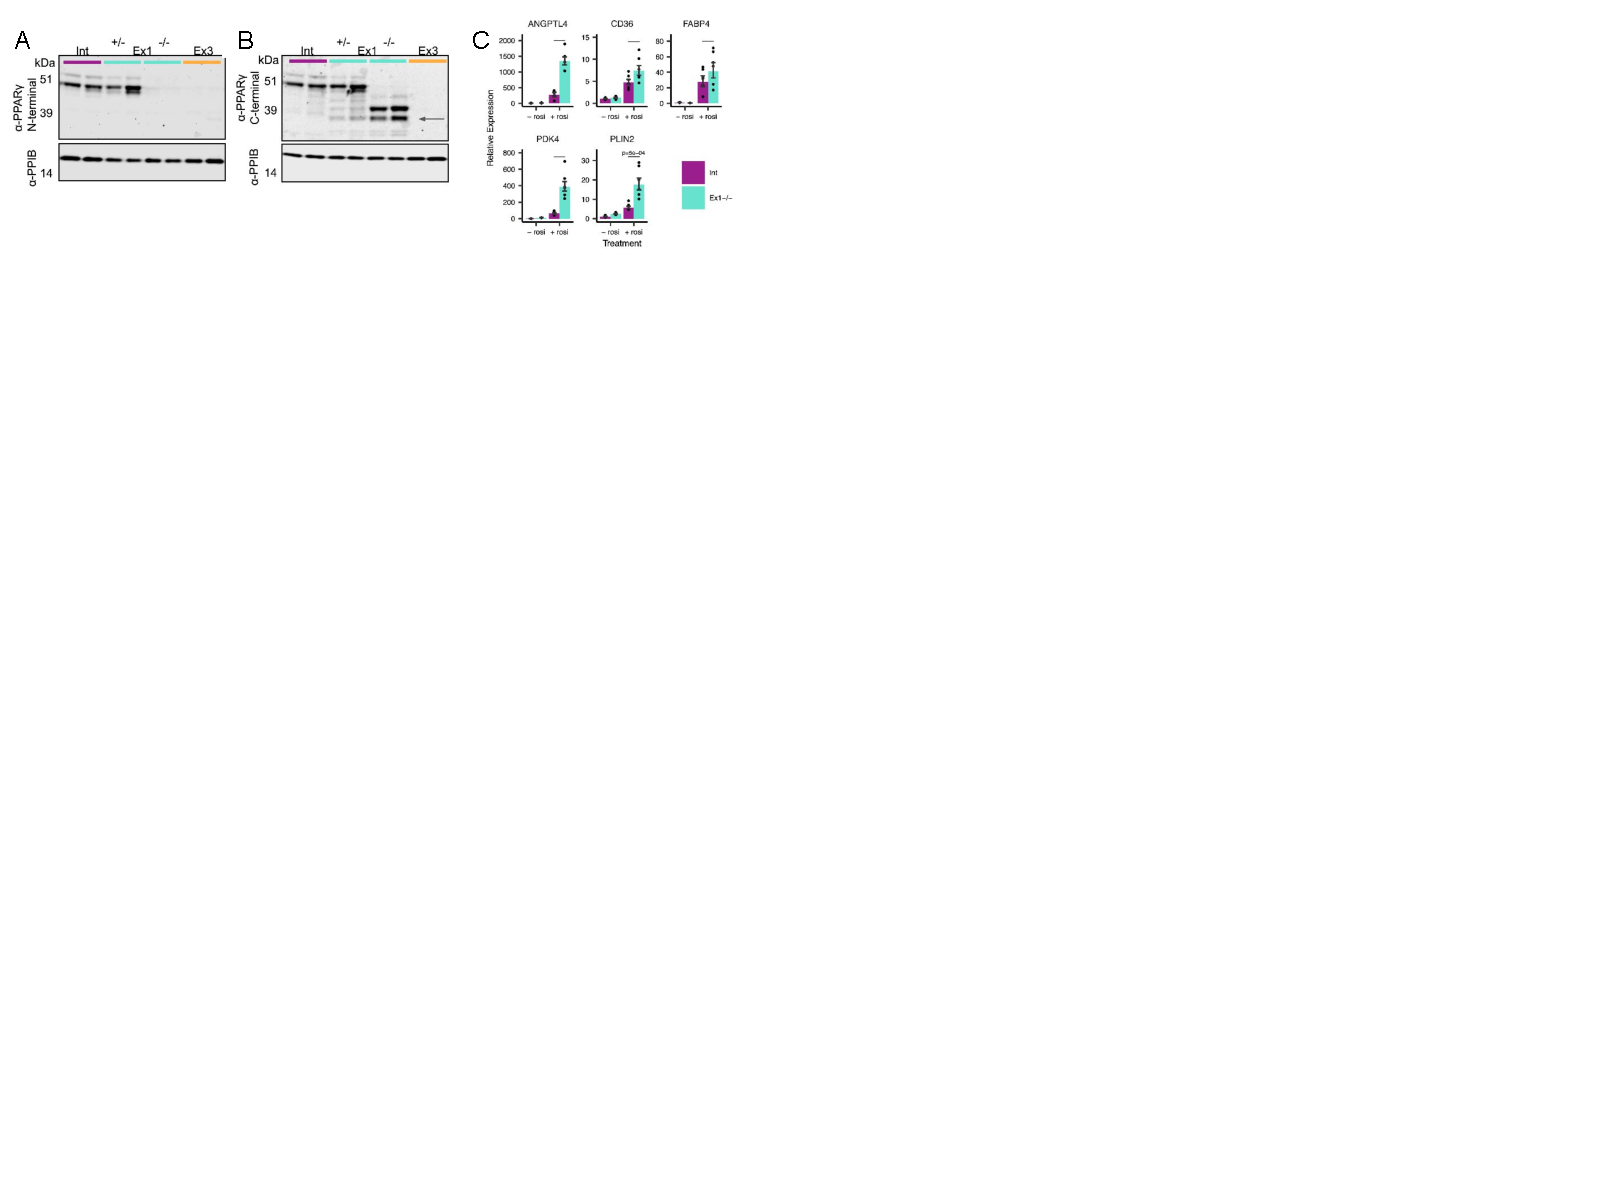
\includegraphics[width=\textwidth]{1_figures-and-files/Fig2.pdf}
    \caption[THP-1 macrophages express a novel isoform of PPAR$\gamma$, named PPAR$\gamma$ M135, when edited upstream of the alternative translational start site.]{\textbf{THP-1 macrophages express a novel isoform of PPAR$\gamma$, named PPAR$\gamma$ M135, when edited upstream of the alternative translational start site.} A. Western blots against the N-terminus and B. C-terminus of PPAR$\gamma$ protein were performed to detect PPAR$\gamma$ isoforms from monoclonal cell lines, evidencing that pre-M135 edited cell lines (Ex1) generate truncated PPAR$\gamma$ bands, including the predicted p.M135 at 40 kDa (arrow) as opposed to post-M135 (Ex3) targeted cell lines and intronic cell lines (Int). C. Relative expression of PPAR$\gamma$ target genes in PPARG targeted monoclonal cell lines, with and without rosiglitazone treatment, with GAPDH as the housekeeping gene and Int-sgRNA edited cells with 0 rosi as control. In response to rosiglitazone, the increases in ANGPTL4, PDK4, and PLIN2 for Ex1 edited cells (n=6, cyan) were greater than the increases in the Int edited cells (n=6, purple) (Welch’s two-sample t-test on delta Ct values). Non-significant increases in CD36 and FABP4 were also observed in Ex1 edited cells.
    }\label{fig:2 THP-1 macrophages can generate novel isoform}
\end{figure}

This 40 kDa band, which was only detected by the C-terminal antibody, had increased intensity in the Ex1-homozygous versus the Ex1-heterozygous cell lines. Some of the other bands detected by the C-terminal antibody could be consistent with translation initiation at AUG codons downstream of the canonical start codon but upstream of p.M135 (e.g. p.M53). Finally, neither the N- or the C-terminal specific antibodies detected protein in the Ex3-sgRNA edited cells, indicating a complete absence of PPAR$\gamma$ protein when Exon 3 is disrupted (\textbf{Figure 1.2B}).

To compare the transcriptional profiles of cells expressing WT and PPAR$\gamma$ M135, the Int-sgRNA +/+ and Ex1-sgRNA -/- clonal cell lines were differentiated into macrophages, stimulated with 1 $\mu$M rosiglitazone and assessed for gene expression at several canonical PPAR$\gamma$ target genes (\textbf{Figure 1.2C}). Upon agonist induction, the Ex1-sgRNA -/- cells expressed significantly higher levels of \(ANGPTL4\)\cite{Aryal2016-ze} (p=0.001), \(PDK4\)\cite{Lefterova2008-rk} (p=6.2e-6), and \(PLIN2\)\cite{Hodgkinson2003-fo} (p=5e-4) than the Int-sgRNA +/+ cells. These PPAR$\gamma$ M135 expressing cells also showed non-significant increases in \(CD36\) and \(FABP4\) expression.

We subsequently isolated and compared the transactivation potentials of WT and PPAR$\gamma$ M135. A PPRE-driven luciferase reporter\cite{Kim1998-aj} and WT PPAR$\gamma$ or PPAR$\gamma$ M135 mRNA were transfected into HEK293s, which have minimal endogenous PPARG activity\cite{Ma2012-dm}. In this system, PPAR$\gamma$ M135 activated transcriptional activity more potently than WT when induced with rosiglitazone (\textbf{Figure A.2a}). We further compared the stability of PPAR$\gamma$ M135 to WT by performing a cycloheximide chase\cite{Hsu1996-yv} in the heterozygous Ex1-sgRNA cells that generate both isoforms (\textbf{Figure A.2b}). The M135 isoform degraded more slowly than PPAR$\gamma$1 (\textbf{Figure A.2c}) which could contribute to its enhanced transactivation potential.

\subsection{Ligand-activated PPAR\texorpdfstring{$\gamma$}{gamma} M135 transactivates target genes more potently than WT PPAR\texorpdfstring{$\gamma$}{gamma} in THP-1s}

We next sought to isolate the activity of PPAR$\gamma$ M135 and evaluate its effect on global transcriptional profiles in comparison with full-length wild-type (WT) PPAR$\gamma$. To compare the direct transcriptional responses of M135 and WT, we performed RNA-seq on PPAR$\gamma$ null (P$\gamma$-/-) THP-1 monocytes electroporated with in vitro transcribed mRNA of each of the two PPAR$\gamma$ isoforms; eGFP mRNA was also electroporated as a process control. In preliminary experiments, mRNA amounts for each isoform were titrated to express similar amounts of protein at the point of harvest (\textbf{Figure A.3}), such that 2 $\mu$g PPAR$\gamma$ M135 mRNA and 8 $\mu$g PPAR$\gamma$ WT were used for each electroporation. The electroporated cells were differentiated into macrophages to mimic the cellular context in which PPAR$\gamma$ is active\cite{Rovera1979-za} and treated with 0 (-) and 1 $\mu$M (+) rosiglitazone. As a positive control, wild-type (P$\gamma$+/+) THP-1 cells with intact \(PPARG\) were also treated with +/- rosiglitazone and transcriptionally profiled (\textbf{Figure 1.3A}).

After filtering for low expression, 16,732 transcripts were retained for analysis across all samples. As expected, rosiglitazone treatment increased gene expression of canonical PPAR$\gamma$ target genes including \(CD36\), \(FABP4\)\cite{Tontonoz1994-nk}, and \(PLIN2\)\cite{Hodgkinson2003-fo} (\textbf{Figure 1.3B}). Remarkably, PPAR$\gamma$ M135-electroporated (P$\gamma$-/- +M135) cells exhibited greater agonist-induced transcriptional responses for some of these targets compared to P$\gamma$-/- +WT or P$\gamma$+/+ THP-1 macrophages, despite comparable PPAR$\gamma$ protein levels (log2 fold-change (log2FC): \(CD36\): P$\gamma$-/- +M135=4.22, P$\gamma$+/+ =2.94, P$\gamma$-/- +WT=1.62. \(PLIN2\): P$\gamma$-/- +M135=3.35, P$\gamma$+/+=3.24, P$\gamma$-/- +WT=1.50).

\clearpage
\begin{figure}[!t]
    \centering
    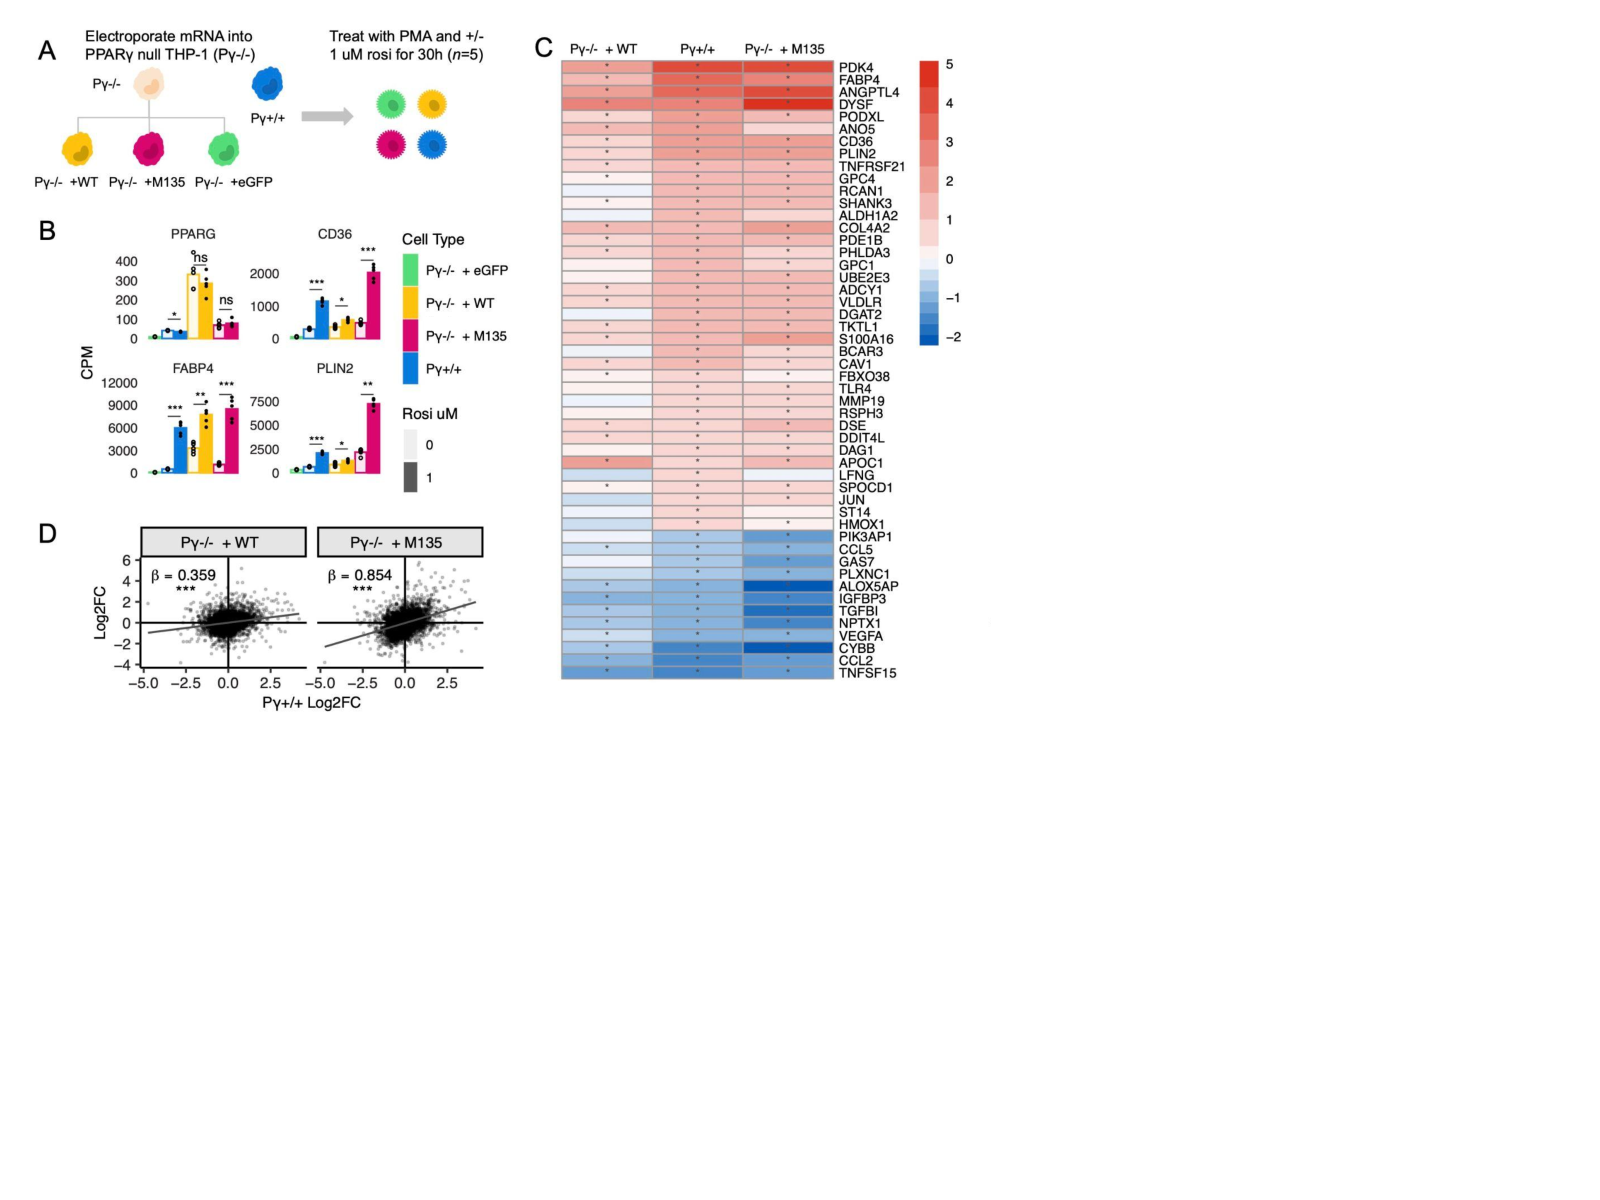
\includegraphics[width=\textwidth]{1_figures-and-files/Fig3.pdf}
    \caption[PPAR$\gamma$ M135 more potently activates ligand stimulated gene expression as compared to WT.]{\textbf{PPAR$\gamma$ M135 more potently activates ligand stimulated gene expression as compared to WT.} A. PPAR$\gamma$ WT and M135 mRNA, along with control eGFP mRNA, were generated through in vitro transcription and electroporated into PPAR$\gamma$ null (P$\gamma$-/-) THP-1 monocytes. The electroporated cells and wild-type THP-1s (P$\gamma$+/+) were differentiated into macrophages and treated with +/- 1 uM rosiglitazone (rosi) for 30 hours before protein and RNA were collected (n=5/condition). B. RNA-seq expression in counts per million (CPM) of PPARG and selected PPAR$\gamma$ target genes. In response to rosiglitazone treatment, P$\gamma$-/- +M135 activates CD36 and PLIN2 with greater fold change than P$\gamma$-/- +WT and P$\gamma$+/+. * Benjamini-Hochberg corrected (BH) p$<$0.01, ** BH p$<$1e-4, *** BH p$<$1e-8. C. Heatmap of log2-fold change (log2FC) in response to rosiglitazone for each cell type of the top 50 differentially expressed genes (DEGs) in P$\gamma$+/+ THP-1s, as ranked by p-value. Asterisks (*) indicate DEGs changing in the same direction with BH corrected p $<$ 0.05. D. Scatterplot of all 1779 P$\gamma$+/+ DEG log2FC values, comparing the log2FC in P$\gamma$+/+ to the log2FC in P$\gamma$-/- +WT and P$\gamma$-/- +M135. Regression slopes ($\beta$) are significant (p $<$ 2e-16, ***) for both, but the P$\gamma$-/- +M135 transcriptional response more closely recapitulates P$\gamma$+/+.
    }\label{fig:3 PPARgamma M135 as a ligand stimulated transactivator}
\end{figure}

To comprehensively evaluate if M135 generated a stronger agonist-induced transcriptional response than WT in P$\gamma$-/- cells, we performed a series of differential expression analyses. We first identified the top-ranked PPAR$\gamma$ target genes as defined by the 50 most significant differentially expressed genes (DEGs) in P$\gamma$+/+ cells +/- rosiglitazone and then compared the log2FC for the same genes across P$\gamma$-/- +WT and P$\gamma$-/- +M135 +/- rosiglitazone (\textbf{Figure 1.3C}). Of the top 50 P$\gamma$+/+ DEGs, 46 were also differentially expressed in P$\gamma$-/- +M135 (p$<$0.05, same sign log2FC), whereas only 33 were differentially expressed in P$\gamma$-/- +WT. Moreover, at several key genes, including \(PDK4\), \(DYSF\), \(ANGPTL4\), \(ALOX5AP\), and \(CYBB\)\cite{De_Morree2013-dh,Pott2012-ji,Keller2018-zv}, P$\gamma$-/- +M135 had a greater activation or repression than P$\gamma$+/+ cells (\textbf{Figure 1.3C}) despite transient and lower PPAR$\gamma$ protein expression per cell (\textbf{Figure A.3}). Across all the P$\gamma$+/+ DEGs (n=1779), the magnitude of gene expression change was more similar for P$\gamma$-/- +M135 cells (slope=0.85) than for P$\gamma$-/- +WT cells (slope=0.36), indicating greater potency of M135 in mediating agonist-induced PPAR$\gamma$ gene expression response than WT (\textbf{Figure 1.3D}).

\begin{figure}[h]
    \centering
    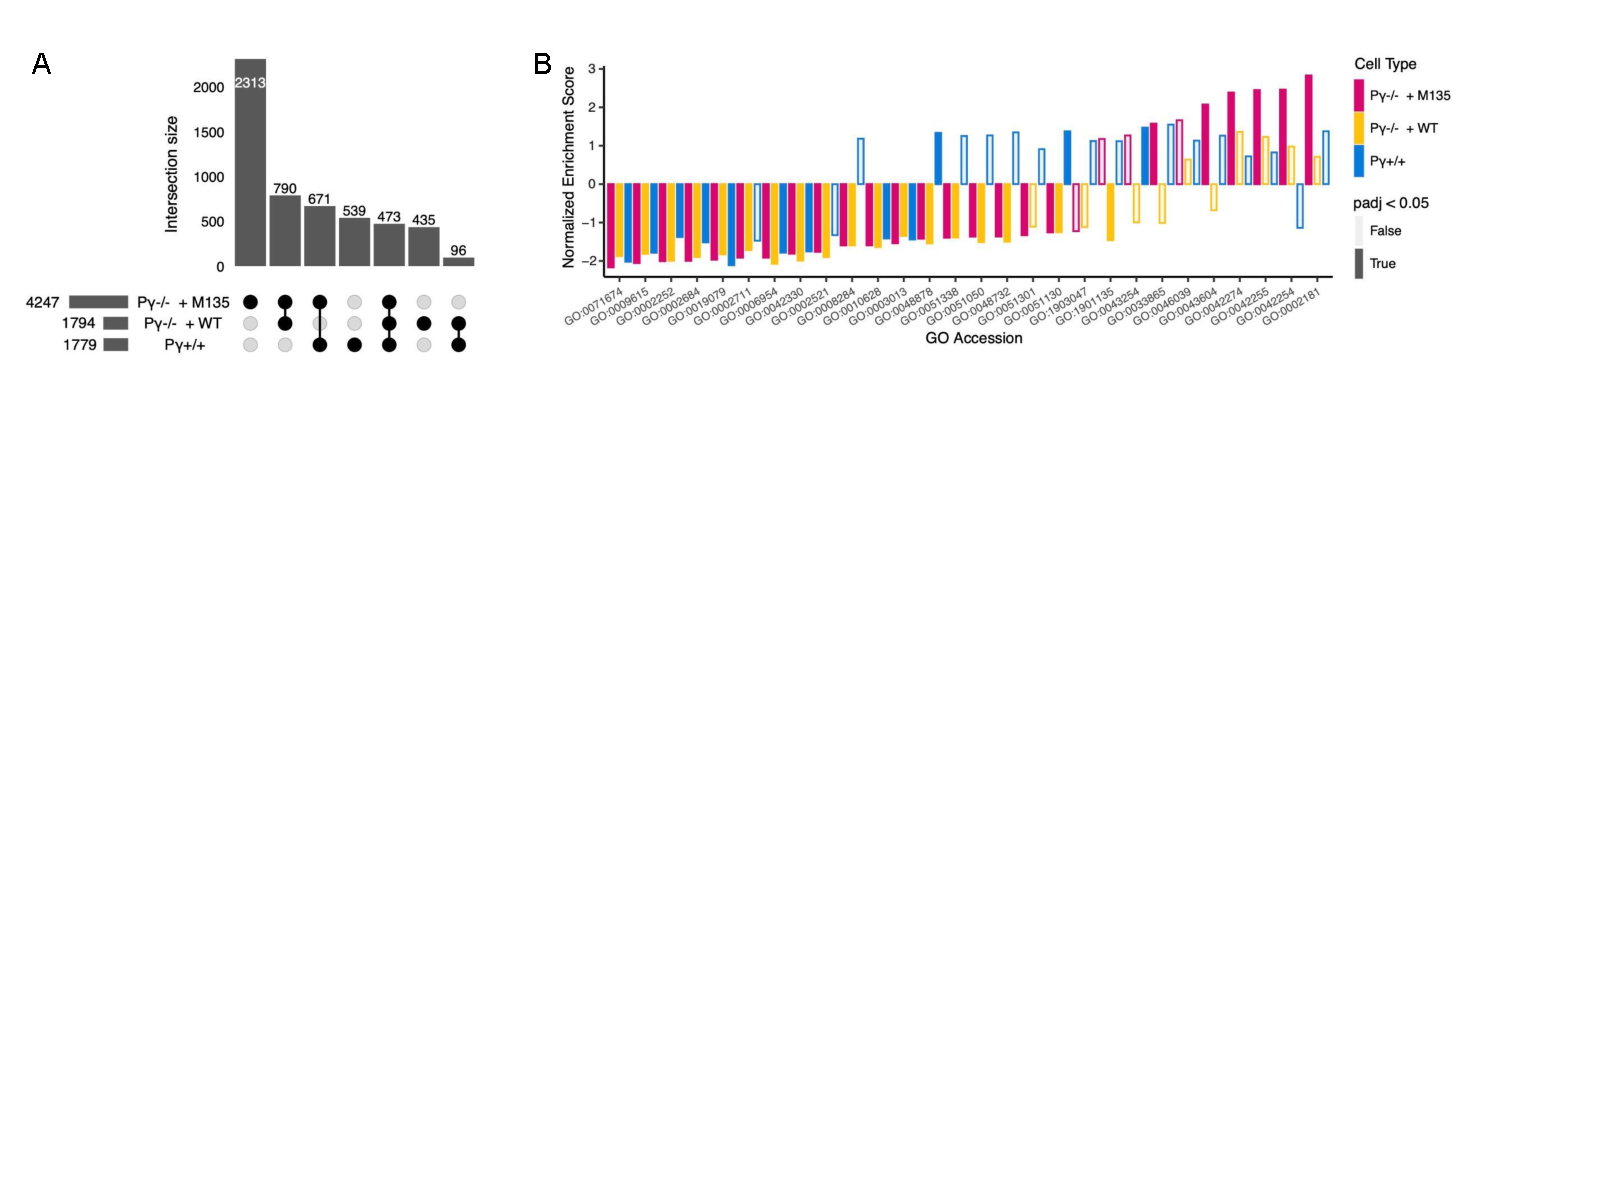
\includegraphics[width=\textwidth]{1_figures-and-files/Fig4.pdf}
    \caption[PPAR$\gamma$ M135 activates more genes in similar biological process pathways as WT.]{\textbf{PPAR$\gamma$ M135 activates more genes in the same biological process pathways as WT.} A. Upset plot of the DEGs per cell type +/- rosiglitazone. Left horizontal bars show total DEGs for each of the three conditions. Filled circles connected by lines indicate intersections among the three conditions and vertical bars show the number of DEGs in the corresponding intersections. B. Normalized enrichment scores in the GO BP pathways for P$\gamma$-/- M135 specific genes. Overall transcriptional pathway activation by P$\gamma$+/+ ,P$\gamma$-/- +WT, P$\gamma$-/- +M135 are similar and consistent.
    }\label{fig:4 PPARgamma M135 has more differentially expressed genes}
\end{figure}

We then queried for DEGs specific to PPAR$\gamma$ M135 to assess if the lack of AF-1 domain in M135 resulted in transactivation/repression of genes not regulated by WT PPAR$\gamma$. In response to rosiglitazone treatment, P$\gamma$-/- +M135 had the greatest number of DEGs (n=4,247, \textbf{Figure 1.4A}) as compared to P$\gamma$-/- +WT (n=1,794) or P$\gamma$+/+ (n=1,779). Of the 4,247 DEGs, 2,313 were exclusive to P$\gamma$-/- +M135 (\textbf{Figure 1.4A}). To understand the gene expression programs captured by these putative M135-specific genes, we performed gene set overrepresentation analysis\cite{Chang2006-im,Yu2012-gb} among the Gene Ontology Biological Process (GO BP) pathways\cite{Ashburner2000-df,Gene_Ontology_Consortium2021-fn} and found 28 overrepresented pathways that were confirmed to be altered by rosiglitazone treatment in M135 complemented cells (p$<$0.05; \textbf{Table A.2}). Among these, 21/28 were similarly altered, although to a lesser degree, by rosiglitazone treatment in either WT-electroporated cells or P$\gamma$+/+ THP-1s (\textbf{Figure 1.4B}). The most enriched result, GO:0002181, is the cytoplasmic translation biological process pathway, and rosiglitazone has been recently found to induce ribosomal transcription in adipocytes\cite{De-Siqueira2024-uz}. Taken together, these analyses suggest that PPAR$\gamma$ M135 regulates similar gene expression programs as WT, but more potently when induced by rosiglitazone, perhaps due to de-repression from the loss of the N-terminal AF-1 domain\cite{Mosure2022-tw}.

%%%%%%%%%%%%%%%%%%%%%%%%%%%%%%%%%%%%%%%%%%%%%%%%%%%%%%%%%%%%%%%%%%%%%%%%%%%%%%%%
\section{Discussion}
%%%%%%%%%%%%%%%%%%%%%%%%%%%%%%%%%%%%%%%%%%%%%%%%%%%%%%%%%%%%%%%%%%%%%%%%%%%%%%%%

In this study, we report and characterize the function of a novel isoform of PPAR$\gamma$ (M135), lacking the AF-1 domain, that can be generated from an alternative downstream translational start site in the second coding exon of \(PPARG\) (chr3:12381414 hg38). We show that PPAR$\gamma$ M135 is transcriptionally active, ligand inducible, and a more potent transactivator than full-length WT PPAR$\gamma$.  

Our finding that PPAR$\gamma$ M135 has increased transactivation potential and is beneficial to metabolic health in vivo aligns with prior studies investigating both naturally occurring and synthetic PPAR$\gamma$ variations. Previous investigators have observed that constructs deleting the N-terminus of PPAR$\gamma$ increase transcriptional potency compared with full-length PPAR$\gamma$ in NIH 3T3 cells\cite{Tontonoz1994-ds,Hummasti2006-rm}. Subsequent work demonstrated that a MAPK phosphorylation site at PPAR$\gamma$ p.S112 inhibits the transactivation function of PPAR$\gamma$\cite{Adams1997-cf}, and PPAR$\gamma$ p.S112A, which lacks the phosphorylation site, is more transcriptionally active\cite{Adams1997-cf,Hu1996-mb,Camp1997-nf}. Additionally, the missense variant PPAR$\gamma$2 p.P12A (rs1801282), which has been robustly associated with a reduced risk of type 2 diabetes in humans\cite{Altshuler2000-kl}, was found to weaken the interaction between PPAR$\gamma$ and its corepressor NCoR, resulting in increased transcriptional activity of PPAR$\gamma$ target genes and improved insulin sensitivity in mice\cite{Heikkinen2009-vb}. Consistent with this mechanism, we find that metabolic syndrome severity scores (METSS) decreases per p.P12A allele carried at the rs1801282 locus. Furthermore, SUMOylation at p.K107 inhibits ligand-induced transactivation of PPAR$\gamma$ targets\cite{Pascual2005-ki}, and removing that modification in mice increased insulin sensitivity without increasing adiposity in mice\cite{Katafuchi2018-jw}. Altogether, these studies illustrate that impairing the AF-1 domain increases PPAR$\gamma$ activity and insulin sensitivity. 

The major limitation of our study is the use of an in vitro cell model. Our experiments were conducted using the THP-1 macrophage cell line which, although human, is not equivalent to in vivo macrophages. However, previous investigations have shown concordant cellular responses between THP-1 monocytes and adipocytes across functional \(PPARG\) variants\cite{Majithia2016-bm,Agostini2018-bx,Majithia2014-op} providing a measure of confidence that these models are suitable for studying genetic variation in \(PPARG\). Furthermore, PPAR$\gamma$ is active in additional tissues including muscle and liver that may have additional metabolic consequences\cite{Norris2003-hi,Gavrilova2003-gb}. These could be the subject of future investigation to fully dissect the metabolic consequences of PPAR$\gamma$ M135.

In summary, we report on PPAR$\gamma$ M135, a novel isoform of \(PPARG\) arising from a downstream alternative translational start site (chr3:12381414 hg38), that is a more potent ligand-inducible transactivator than full-length PPAR$\gamma$. This work points to a new mechanism to activate PPAR$\gamma$ by inhibition of the AF-1 domain that could potentially lead to more effective treatments for insulin resistance-related disorders.

%%%%%%%%%%%%%%%%%%%%%%%%%%%%%%%%%%%%%%%%%%%%%%%%%%%%%%%%%%%%%%%%%%%%%%%%%%%%%%%%
\section{Research Design and Methods}
%%%%%%%%%%%%%%%%%%%%%%%%%%%%%%%%%%%%%%%%%%%%%%%%%%%%%%%%%%%%%%%%%%%%%%%%%%%%%%%%

\subsection{Cell Culture}
Cell suspensions from the human monocytic leukemia cell line THP-1 (ATCC \#TIB-202) were cultured in growth media (RPMI 1640 (Gibco, \#22400089) + 10\% heat-inactivated FBS (Sigma- Aldrich, \#F2442) + 1\% PenStrep (Gibco, \#15140122) + 0.1\% 2-Mercaptoethanol (BME; Sigma-Aldrich, \#M6250)). In all experiments, cells were differentiated with 50 ng/mL phorbol 12-myristate 13-acetate (PMA; Sigma-Aldrich, \#P1585) and PPAR$\gamma$ activation was stimulated with 1uM rosiglitazone (Cayman Chemicals, \#71740).

\subsection{Generation of the pooled CRISPR library}
To study the effect of insertions and deletions (indels) across \(PPARG\), guide RNAs (sgRNAs) were designed using CRISPick\cite{Doench2016-za}, ordered as premixed oligos from IDT, phosphorylated, annealed, and ligated into the lentiCRISPRv2 vector (Addgene \#52961) through Golden Gate cloning\cite{Engler2008-in}. The plasmids were transformed and sequenced for verification. Lentivirus was generated following manufacturer protocols (Mirus Bio \#2304) and used to infect THP-1 cells at MOI=0.3 to minimize doubly infected cells, and the edited cells were selected for using 2 $\mu$g/mL puromycin (Sigma-Aldrich, \#P8833). The distribution and efficiency of infection were assessed as follows. Genomic DNA (gDNA) was extracted from 1 million cells (Qiagen \#51304), split across 4 PCR reactions, amplified (Takara 639208), and loaded onto the iSeq (Illumina), and the reads were deconvolved with PoolQ 3.3.2 (Broad Institute; \url{https://portals.broadinstitute.org/gpp/public/software/poolq}), which showed a 96.8\% completeness with a maximum of 100x difference between the most over-sequenced guide and the least.

\subsection{Pooled CRISPR experimental assay}
To assess the effect of indels across \(PPARG\) on its ability to activate a downstream target, the edited THP-1 cells were sorted, alongside wildtype (P$\gamma$+/+) THP-1s and PPAR$\gamma$ null (P$\gamma$-/-) THP-1s, for expression of CD36. To activate PPAR$\gamma$, the cells were treated with 50 ng/mL PMA for 72 hours and 1 $\mu$M rosiglitazone for 48 hours. The cells were immunostained for CD36 (Miltenyi Biotec, \#130-095-472). Stained cells were sorted using FACS (BD FACSAria II) into two bins: high and low expression of CD36, based on thresholds set by the P$\gamma$+/+ and P$\gamma$-/- cells. 5 independent sorting experiments were performed, sorting approximately 150,000 cells per bin per replicate. To identify and quantify the \(PPARG\) variants in each bin, the methods detailed above were used to extract gDNA, amplify, and sequence. To quantify the effect of each sgRNA on PPAR$\gamma$ function, an enrichment score was generated. The reads for each sorted sample were normalized by library depth, and enrichment was calculated by taking the log2 of the ratio of CD36+ normalized counts to CD36- normalized counts for each sgRNA. 

\subsection{Saturation mutagenesis frameshift analysis}
To determine the impact of indels at each codon of \(PPARG\), a function score for each codon was calculated based on previously published methods\cite{Majithia2016-bm}. The function score is analogous to the CD36+/CD36- enrichment score described above.

\subsection{Generation of monoclonal cell lines}
The endonuclease Cas9 and guides Int-sgRNA, Ex1-sgRNA, and Ex3-sgRNA (\textbf{Table A.1}) were introduced into THP-1 cells by lentiviral transduction. The transduced THP-1 cells were sorted one cell per well into 96-well plates (BD FACSAria II) in growth media supplemented with 50\% conditioned media (RPMI media harvested from healthy cells at $\sim$70\% confluence for 48 hours post the previous passage, clarified by centrifugation at 1000 x g for 10 minutes and then passed through a 0.2 $\mu$m sterile filter to remove any cell debris) and expanded. All cell lines were sequenced to confirm genomic edits and zygosity by Sanger sequencing of genomic DNA.

\subsection{Detecting PPAR\texorpdfstring{$\gamma$}{gamma} isoforms}
Cells were lysed using RIPA lysis buffer (Millipore Sigma, \#20-188), and protease inhibitor (Roche, \#04693132001), and protein concentration was determined. Equal amounts of proteins were separated by 4-12\% Bis-Tris Gels (Invitrogen, \#NP0336) with the SeeBlue Plus2 Prestained Protein Standard (Invitrogen, LC5925) and subsequently blotted on 0.45 um nitrocellulose membrane (Bio-Rad, \#1620115). The membrane was incubated with antibodies against PPAR$\gamma$ for N-terminus (1:1000 Cell Signaling Technology (CST) \#2435, RRID:AB\_2166051), for C-terminus recognition (1:1000 CST \#2443, RRID:AB\_823598), and cyclophilin B (1:1000 CST Cat\# 43603, RRID:AB\_2799247), followed by anti-rabbit secondary antibody conjugated with DyLight 680 Fluorescent dye (1:20,000 CST \#5366, RRID:AB\_10693812). Finally, the membranes were visualized with Odyssey CLx imager (LI-COR).

\subsection{Cycloheximide chase}
3 million THP-1 cells were seeded per well in a 6-well plate and differentiated for 24 hours with 50 ng/mL PMA. Translation was arrested with 5 uM cycloheximide, and cells were collected after 0, 0.5, 1, and 2 hours of treatment (n=3). Fifteen $\mu$g protein from each sample were loaded into a western blot with the PageRuler Plus Prestained Protein Ladder (Thermo \#26619) and processed as detailed above with primary antibodies CST \#2443 for PPAR$\gamma$ and CST \#41185 for actin. Intensities for the PPAR$\gamma$1, PPAR$\gamma$ M135, and actin bands were quantified on Image Studio, and the PPAR$\gamma$ intensities for each sample were normalized to its corresponding actin intensity to control for the amount of protein. For each PPAR$\gamma$ isoform, the percentage relative to baseline was calculated by dividing the normalized PPAR$\gamma$ intensity by the mean of that isoform at 0 hours. For each sample, the ratio of PPAR$\gamma$1 to PPAR$\gamma$ M135 was obtained by dividing the percentage relative to baseline of PPAR$\gamma$1 by that of PPAR$\gamma$ M135. Statistical analysis was performed with one-way ANOVA with a Tukey post hoc test.

\subsection{In vitro transcription}
To evaluate the complementation of PPAR$\gamma$ using wildtype (WT) and M135 PPAR$\gamma$ isoforms, in vitro transcription was performed as previously described\cite{Heinz2018-mp}. Briefly, cDNA constructs were amplified from plasmids containing the PPAR$\gamma$2 sequence using primers that introduce a T7 promoter and AG on the 5$^{\prime}$ end and a 179-nt poly (A) on the 3$^{\prime}$ end (PPAR$\gamma$ WT FWD: 5$^{\prime}$-GAATTTAATACGACTCACTATAAGGAAATACGCCACCATGGGTGAAACTCTGGGAGAT-3$^{\prime}$; M135 FWD: 5$^{\prime}$-GAATTTAATACGACTCACTATAAGGAAATACGCCACCATGGCAATTG\newline AATGTCGTGTCT-3$^{\prime}$, REV1: 5$^{\prime}$-CTAGGACATCGCAGTCTGCACCTAGTACAAGTCCTTG\newline TAGATCTCCTG-3$^{\prime}$; REV2: 5$^{\prime}$- (T)179-CTAGGACATCGCAGTCTGCAC-3$^{\prime}$). To generate capped, polyadenylated mRNA, PCR products were phenol-chloroform extracted and in vitro transcribed with T7 RNA Polymerase HiScribe Mix (NEB \#E2040S), CleanCap Reagent AG (TriLink \#N-7113) and 5-methoxyuridine triphosphate (TriLink \#N-1093-5) instead of UTP. The mRNA was precipitated with lithium chloride and resuspended in water.

\subsection{Luciferase assay}
Transcriptional activity of the PPAR$\gamma$ isoforms was tested in HEK293 cells using a PPAR promoter driven luciferase reporter (PPREx3-luc, Addgene plasmid \# 1015; a gift from Bruce Spiegelman). HEK293 cells were seeded 20,000/well and co-transfected with a mixture of 10 ng Renilla (pGL4.75), 10 ng PPREx3-LUC, and 100 ng PPAR$\gamma$ mRNA using Lipofectamine 3000 (Thermo L3000001) for 48 hours. Rosiglitazone treated samples were incubated with 0.5 uM for 16 hours. Firefly and Renilla luciferase activity was quantified by using the Dual Luciferase Assay System (Promega \#E1910), as described by the manufacturer. Luciferase activity was normalized for moles of mRNA transfected.

\subsection{Creating THP-1 cells with exogenous isoforms}
To introduce the \(PPARG\) IVT mRNA into P$\gamma$-/- THP-1 cells, the transcripts were electroporated into cells on the BioRad XCell in a 4 mm cuvette with one 400 V, 5 ms square wave pulse. To match PPAR$\gamma$ protein expression, 2 $\mu$g of M135 mRNA and 8 $\mu$g of WT mRNA were used for each electroporation of 3 million cells (n=5 per cell type). After each electroporation, the cells were split into 3 for protein collection, treatment with 50 ng/uL PMA, and treatment with 50 ng/uL PMA and 1 $\mu$M rosiglitazone. To study the transcriptomes of these cells, RNA was extracted from the latter two conditions (Zymo \#R1050) and sent for library preparation (Illumina Stranded mRNA Prep) and 100 bp paired-end sequencing (25 million reads/sample on the NovaSeq S4).

\subsection{Transcriptomic analysis of THP-1 cell types}
 Raw sequencing reads were aligned to the reference hg38 using Kallisto with default parameters\cite{Bray2016-zt} to generate gene counts per cell. Analysis was performed in R 4.1.3. EdgeR 3.36.0 and limma-voom (limma v3.50.1) were used to filter and normalize reads for library size and perform differential expression\cite{Robinson2010-qx,Law2014-yh}. UpSetR v1.4.0 was applied to visualize the intersections in differentially expressed genes (DEGs) between the P$\gamma$+/+, P$\gamma$-/- +M135, and P$\gamma$-/- +WT cell lines in response to rosiglitazone\cite{Lex2014-lr,Conway2017-hp}. To study changes in gene sets, overrepresentation analyses and enrichment analyses were performed in fgsea v1.20.0\cite{Korotkevich2021-ra}.

\subsection{Treatment of monoclonal THP-1 cells for qPCR}
Ex1-sgRNA -/- and Int-sgRNA +/+ monoclonal cells were seeded in 12-well plates with 750,000 cells per well. 12 wells of each genotype were differentiated with 50 ng/mL PMA for a total of 72 hours, with 6 wells of each genotype additionally receiving 1 uM rosiglitazone in the last 24 hours. RNA was extracted (Zymo \#R1050) for qPCR. Two independent rounds of seeding and collection were performed.

\subsection{Quantitative PCR for THP-1s}
Reverse transcription was performed with the SuperScript III First-Strand Synthesis System (ThermoFisher 18080051) following manufacturer’s instructions. Gene expression was analyzed using the iTaq Universal SYBR Green Supermix (Bio-Rad 1725121) with \(GAPDH\) as the housekeeping gene. Cycle threshold values (Ct) were analyzed using the $\Delta\Delta$Ct method\cite{Livak2001-va}. Briefly, following outlier removal, technical replicates (n=2) were averaged, and $\Delta$Ct values were calculated for each biological replicate along with their mean and standard error (n=6 for Figure 1.2C). Relative expression (fold-change) was calculated as \[2^{-\Delta\Delta Ct}\] setting a reference condition $\Delta$Ct from differentiated Int-sgRNA THP-1s as a calibrator.

%%%%%%%%%%%%%%%%%%%%%%%%%%%%%%%%%%%%%%%%%%%%%%%%%%%%%%%%%%%%%%%%%%%%%%%%%%%%%%%%
\section{Acknowledgements}
%%%%%%%%%%%%%%%%%%%%%%%%%%%%%%%%%%%%%%%%%%%%%%%%%%%%%%%%%%%%%%%%%%%%%%%%%%%%%%%%

We are deeply grateful to Angela Liu for technical assistance. 
 
\subsection{Author Contributions}
A.R.M conceived the study. X.D., K.M.-L., and A.R.M. designed the experiments. X.D., K.M-L., S.H., R.D., G.B., R.H., K.G., C.D.A.S., J.F., S.Heinz and A.R.M. generated/acquired and analyzed the data. X.D., K.M.-L., S.H., R.D., G.B., R.H., J.F., S.Heinz, and A.R.M. were involved in data interpretation. X.D., K.M-L. and A.R.M. drafted the initial manuscript. All authors were involved in manuscript revision. A.R.M is the guarantor of this work and, as such, had full access to all the data in the study and takes responsibility for the integrity of the data and the accuracy of the data analysis.

\subsection{Duality of Interest}
The authors declare no competing interests.  

\subsection{Funding}
This work was supported by grants from the National Institute of Diabetes and Digestive and Kidney Diseases (1R01DK123422 and R01HL159760 to A.R.M, 1R01DK125490 to J.F and A.R.M) and a UCSD/UCLA Pilot and Feasibility grant (P30 DK063491 to A.R.M). This publication includes data generated at the UC San Diego IGM Genomics Center utilizing an Illumina NovaSeq 6000 that was purchased with funding from a National Institutes of Health SIG grant (\#S10 OD026929).\\ 

\noindent Chapter 1, in full, was modified for this thesis from the material in Diabetes 2025. The dissertation/thesis author was the primary investigator and author of this paper. I would like to acknowledge my co-authors for the research in Chapter 1, Karen Mendez-Lara, Siqi Hu, Rachel Diao, Guru Bhavimani, Ruben Hernandez, Kimberly Glass, Camila De Arruda Saldanha, Jason Flannick, Sven Heinz, and Amit Majithia.

\bibliographystyle{unsrtnat}
\bibliography{bib_1.bib}